%% Dokumentklasse KOMA-Script Report
\documentclass[paper=a4, 12pt]{scrreprt}
%% Encoding UTF8
\usepackage[utf8]{inputenc}
%%Use Source Sans Pro Textstyle
\usepackage[default]{sourcesanspro}
%% 8 Bit Aufloesung der Buchstaben
\usepackage[T1]{fontenc}
%% Seitenraender
%\usepackage[scale=0.72]{geometry}
\usepackage[scale=0.72, twoside, bindingoffset=2mm]{geometry}
%% Spracheinstellungen
\usepackage[english, naustrian]{babel} % your native language must be the last one!!
%% erweiterte Farbenpalette
\usepackage[dvipsnames]{xcolor}
%% Abbildungen
\usepackage{graphicx}
%%Tabelen mit Farbe (cellcolor)
\usepackage{tabulary}
\usepackage{colortbl}
\PassOptionsToPackage{dvipsnames,svgnames,table}{xcolor}
%% Tabellen (erweitert)
\usepackage{tabularx}
%% TikZ + Circuit-TikZ (fuer Schaltungen)
\usepackage[europeanresistors, europeaninductors]{circuitikz}
%% Nuetzliche TikZ Libraries
\usetikzlibrary{arrows, automata, positioning}
%% mathematik
\usepackage{amsmath, amssymb}
%%Formelbeschreibung
\newenvironment{conditions}
  {\par\vspace{\abovedisplayskip}\noindent\begin{tabular}{>{$}l<{$} @{${}...{}$} l}}
  {\end{tabular}\par\vspace{\belowdisplayskip}}
%\usepackage{mathtools}	
%% pdf-einbindung
\usepackage{pdfpages}
%% scource-code einbindung
\usepackage{listings, scrhack} %scrhack vermeidet Umschaltung auf KOMA
% Floats..
\usepackage{courier}
%% euro-symbol
\usepackage{eurosym}
%% landcsape-seiten ermöglichen
\usepackage{lscape}

%% Diplomarbeits-Format
\usepackage{srdpdipa}

%% Abkuerzungsverzeichnis
\usepackage[]{acronym}

%% Todos
\usepackage[]{todonotes}

%% Ganttdiagramme
\usepackage{pgfgantt}

%% Subfigures
\usepackage[lofdepth]{subfig}

%% Für Quellenangaben unter Bildern
\newcommand*{\quelle}[1]{\par\raggedleft\footnotesize Quelle:~#1}

%% Listings (Code)
\usepackage{listings}
\usepackage{color}

\definecolor{dkgreen}{rgb}{0,0.6,0}
\definecolor{gray}{rgb}{0.5,0.5,0.5}
\definecolor{mauve}{rgb}{0.58,0,0.82}

\lstset{frame=none,
  language=Python,
  aboveskip=3mm,
  belowskip=3mm,
  showstringspaces=false,
  columns=flexible,
  basicstyle={\small\ttfamily},
  numbers=left,
  numberstyle=\tiny\color{gray},
  keywordstyle=\color{blue},
  commentstyle=\color{dkgreen},
  stringstyle=\color{mauve},
  breaklines=true,
  breakatwhitespace=true,
  tabsize=3
}

\lstset{literate=%
  {Ö}{{\"O}}1
  {Ä}{{\"A}}1
  {Ü}{{\"U}}1
  {ß}{{\ss}}1
  {ü}{{\"u}}1
  {ä}{{\"a}}1
  {ö}{{\"o}}1
}

%% TIKZ Flowcharts
\usepackage{tikz}
\usetikzlibrary{shapes.geometric, arrows}

\tikzstyle{startstop} = [rectangle, rounded corners, minimum width=3cm, minimum height=1cm,text centered, draw=black, fill=green!32]
\tikzstyle{io} = [trapezium, trapezium left angle=70, trapezium right angle=110, minimum width=3cm, minimum height=1cm, text centered, draw=black, fill=red!35]
\tikzstyle{process} = [rectangle, minimum width=3cm, minimum height=1cm, text centered, draw=black, fill=cyan!32]
\tikzstyle{decision} = [diamond, minimum width=3cm, minimum height=1cm, text centered, draw=black, fill=orange!42]

\tikzstyle{arrow} = [thick,->,>=stealth]


%% definitionen =====================================%%
\dataSchool{HTBLuVA St. Pölten}
\dataDepartment{Höhere Lehranstalt für Elektronik und Technische Informatik}
\dataSubdepartment{Ausbildungsschwerpunkte Embedded- \& Wireless Systems}
\dataSession{2024/25}


\title{AirSens Classroom Data Capturing}
\author{Thomas Potzmader \and Tobias Geppl}
\date{4. April 2025}
\place{St. P\"olten}
\professor{Dipl.-Ing. Wolfgang Uriel Kuran \and DI (FH) Johannes Tomitsch}



%%====================================================%%

% Hyperlinks im Dokument
\usepackage[colorlinks=true,
    linkcolor=black,
    citecolor=black,
    bookmarks=true,
    urlcolor=black,
    bookmarksopen=true]{hyperref}

\begin{document}

\frontmatter

%% titelseite ==========================================%%
\maketitle
%%======================================================%%

%% komplett leere seite ================================%%
\newpage\null\thispagestyle{empty}%\newpage
%%======================================================%%

%% eidesstattliche erklärung ===========================%%
\begin{affidavit}
    \unterschrift{Thomas Potzmader}
    \unterschrift{Tobias Geppl}
\end{affidavit}
%%======================================================%%

%% dokumentation (deutsch/englisch) ====================%%
%%\includepdf[pages=-]{doc/pdfs/dokumentation-de.pdf}                 %Dokumentation(PDF) einfügen
%%\includepdf[pages=-]{doc/pdfs/dokumentation-en.pdf}                 %Dokumentation(PDF) einfügen
%%======================================================%%

\cleardoublepage                                              %Seite freilassen


%% diplomantenvorstellung ==============================%%
%%\includepdf[pages=-]{doc/pdfs/Tobias.pdf}                          %Vorstellung(PDF) einfügen
%%\cleardoublepage                                              %Seite freilassen
%%\includepdf[pages=-]{doc/pdfs/Thomas.pdf}                          %Vorstellung(PDF) einfügen
%%======================================================%%

%%\cleardoublepage                                              %Seite freilassen

%% danksagung ==========================================%%
\begin{acknowledgements}
\subsubsection*{Name 1}
Danksagung Inhalt
\\
Danke Danke Danke Danke Danke Danke Danke Danke Danke Danke Danke Danke Danke Danke Danke Danke 
\\                              %Absatz
\subsubsection*{Name 2}
Danksagung Inhalt
\\
Danke Danke Danke Danke Danke Danke Danke Danke Danke Danke Danke Danke Danke Danke 
\end{acknowledgements}
                             
%%======================================================%%

%%\cleardoublepage                                              %Seite freilassen

%% inhaltsverzeichnis ==================================%%
\renewcommand*\chapterpagestyle{scrheadings}
\tableofcontents
%%======================================================%%

%%\cleardoublepage                                              %Seite freilassen

%% HAUPTTEIL ===========================================%%
\responsible{Name 1, Name 2}
\mainmatter

%Chapter 1 - Einführung/Einleitung
\responsible{Thomas Potzmader, Tobias Geppl} 
\begin{inhalt}
\renewcommand*\chapterpagestyle{scrheadings}
\chapter{Einleitung}
Zielsetzung Aufgabenstellung des Gesamtprojekts

Individuelle Zielsetzung und Aufgabenstellung



\section{Section}
Inhalt

\begin{figure}[!htb]
\centering
\includegraphics[width=0.75\textwidth]{img/Quest1.jpg}
\caption[Bildbezeichnung für Abbildungsverzeichnis]{Bildunterschrift}
\label{labelname}
\end{figure}

Inhalt 2

\end{inhalt}                                     %Einführung(LaTeX File) einfügen

%Chapter 2 - Grundlagen (& Methoden)
\responsible{Thomas Potzmader, Tobias Geppl} 
\begin{inhalt}
\renewcommand*\chapterpagestyle{scrheadings}
\chapter{Grundlagen}



\end{inhalt}                                      %Grundlagen(LaTeX File) einfügen

%Chapter 3 - (Methoden)
\responsible{Thomas Potzmader, Tobias Geppl} 
\begin{inhalt}
\renewcommand*\chapterpagestyle{scrheadings}
\chapter{Methoden}


\end{inhalt}                                      %Methoden(LaTeX File) einfügen

%Chapter 4 Ergebnisse
\responsible{Thomas Potzmader, Tobias Geppl} 
\begin{inhalt}
\renewcommand*\chapterpagestyle{scrheadings}
\chapter{Ergebnisse}






\end{inhalt}                                      %Ergebnisse(LaTeX File) einfügen


%Chapter 5 Hardwareentwicklung
\responsible{Tobias Geppl} 
\begin{inhalt}
\renewcommand*\chapterpagestyle{scrheadings}
\chapter{Hardwareentwicklung}

Einführung in Tobias Teil Kurze Erklärung
\section{Komponentenwahl}
\subsection{Sensoren}
\subsection{Mikrocontroller}
\subsection{Bedienelemente}





\section{Versorgungen \& Ansteuerungen}
\subsection{Bussysteme}
\subsection{Spannungsversorgungen}

\section{Pin-Layout \& Schematik}


\section{PCB-Design}


\end{inhalt}                                      

%Chapter 6 Mikrocontroller-Programmierung
\responsible{Tobias Geppl} 
\begin{inhalt}
\renewcommand*\chapterpagestyle{scrheadings}

\chapter{Mikrocontroller-Programmierung}

Die Programmierung des Raspberry Pi Pico W erfolgte mithilfe der Entwicklungsumgebung Visual Studio Code (Kap. \ref{sec:VS-Code}) in Kombination mit der Raspberry Pi Pico-Erweiterung (Kap. \ref{sec:PicoExtension}). Als Programmiersprache wurde C/C++ verwendet. Die Projektstruktur basierte auf dem CMake-Buildsystem mit der Verwendung des offiziellen Pico SDK (\ref{…}). 

\section{I2C:} \label{I2C_Programmierung}

Der Raspberry Pico W besitzt zwei I2C-instanzen: i2c0 und i2c1. Bei der Initialisierungsfunktion i2c\_init(), muss die I2C-Instanz sowie die Taktgeschwindigkeit übergeben werden. Diese Funktion wird von dem Pico SDK (\ref{….}) bereitgestellt. 

\begin{lstlisting} [style=mytsx]
i2c_init(i2c0, 100 * 1000); // i2c0 mit 100 kHz Takt initialisieren
\end{lstlisting}
\index{Code Snippet 1@\hyperref[code:snippet1]{Snippet 1}}


Anschließend werden die entsprechenden GPIO-Pins sowie die internen Pullup-Widerstände gesetzt, da sich keine physischen Pullup-Widerstände auf den Leitungen befinden. 

\\bigskip \\


\textbf{Schreiben:}

Um Daten auf den I2C-Bus zu schreiben, wird folgende Funktion benutzt:

\begin{lstlisting} [style=mytsx]
int i2c_write_blocking(i2c_inst_t *i2c, uint8_t addr, const uint8_t *src, size_t len, bool nostop);
\end{lstlisting}
\index{Code Snippet 1@\hyperref[code:snippet1]{Snippet 1}}

\begin{table}[H]
\centering
\renewcommand{\arraystretch}{1.3}
\begin{tabular}{|l|p{10cm}|}
\hline
\rowcolor{cyan!20}
\textbf{Parameter} & \textbf{Bedeutung} \\
\hline
\texttt{i2c} & I²C-Instanz (\texttt{i2c0} oder \texttt{i2c1}) \\
\hline
\texttt{addr} & I²C-Adresse des Slaves \\
\hline
\texttt{src} & Zeiger auf das zu sendende Datenarray \\
\hline
\texttt{len} & Anzahl der zu sendenden Bytes \\
\hline
\texttt{nostop} & \texttt{false} = STOP \newline
\texttt{true} = REPEATED START \\
\hline
\end{tabular}
\caption{I2C-Sende-Funktion Parameterübersicht}
\label{tab:i2c_parameter}
\end{table}




\textbf{Lesen:}

Um Daten vom I2C-Bus zu lesen, wird folgende Funktion benutzt:

\begin{lstlisting} [style=mytsx][caption={I2C Initialisierung}, label={code:i2c_init}]
int i2c_read_blocking(i2c_inst_t *i2c, uint8_t addr, uint8_t *dst, size_t len, bool nostop);
\end{lstlisting}
\index{Code Snippet 1@\hyperref[code:snippet1]{Snippet 1}}

\begin{table}[H]
\centering
\renewcommand{\arraystretch}{1.3}
\begin{tabular}{|l|p{10cm}|}
\hline
\rowcolor{cyan!20}
\textbf{Parameter} & \textbf{Bedeutung} \\
\hline
\texttt{i2c} & I2C-Instanz (\texttt{i2c0} oder \texttt{i2c1}) \\
\hline
\texttt{addr} & I2C-Adresse des Slaves \\
\hline
\texttt{dst} & Zielpuffer für empfangene Bytes \\
\hline
\texttt{len} & Anzahl der zu lesenden Bytes \\
\hline
\texttt{nostop} & Meist \texttt{false}, es sei denn, ein \texttt{REPEATED START} ist erforderlich \\
\hline
\end{tabular}
\caption{I2C-Lese-Funktion Parameterübersicht}
\label{tab:i2c_read_parameters}
\end{table}

Beim Lesen muss zuerst das entsprechende Register geschrieben werden, um anschließend die Daten daraus auszulesen. 

\bigskip \\
Die Lese- und Schreibfunktionen werden vom Pico SDK bereitgestellt.

\textbf{I2C-Beispiel:}

Als Beispiel wurde vom Host die Daten 0xAA an den Slave mit der Adresse 0x28 gesendet. 

\begin{lstlisting} [style=mytsx][caption={I2C Initialisierung}, label={code:i2c_init}]
test_buffer[0] = 0xAA;
i2c_write_blocking(i2c, 0x28, test_buffer, 1, false);
\end{lstlisting}
\index{Code Snippet 1@\hyperref[code:snippet1]{Snippet 1}}

\begin{figure}[!htb]
\centering
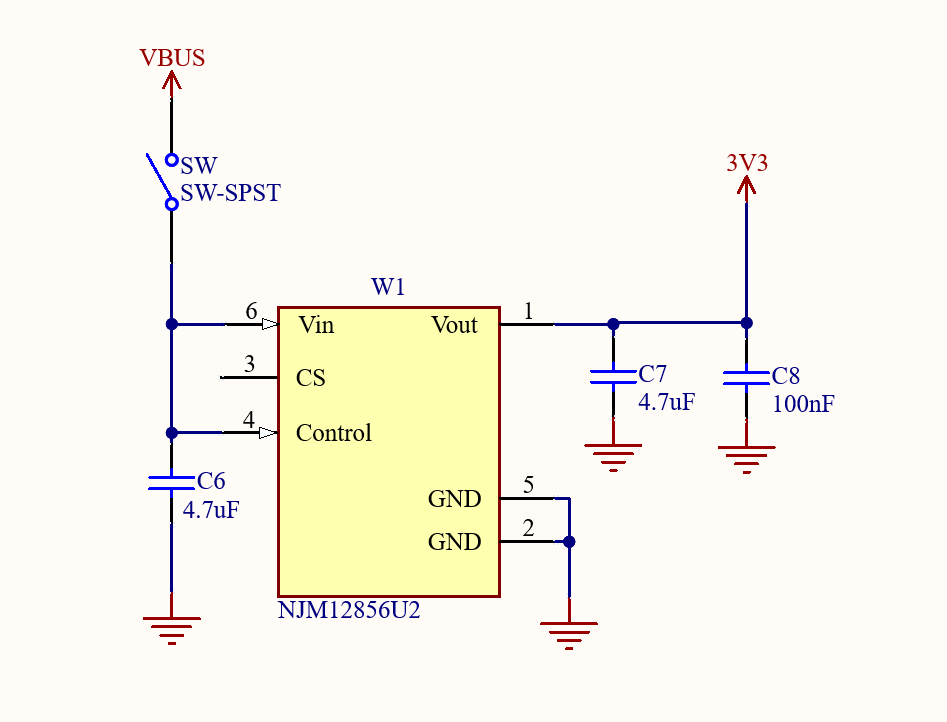
\includegraphics[width=0.75\textwidth]{files/Tobias/pics/Schaltungen/Schematik/3V3_Converter_Schematik.PNG}
\caption[3,3V Spannungsregler Schematik]{3,3V Spannungsregler Schematik}
\label{fig:3,3V Spannungsregler Schematik}
\end{figure}



\section{PAS CO2}

Da für den PAS CO2-Sensor keine Bibliotheken speziell für den Raspberry Pi Pico W verfügbar sind, wurde mithilfe des Datenblatts \cite{Raspberry_Pi_Pico_W} sowie des Programming-Guides \cite{PASCO2_ProgrammingGuide} des PAS CO2 eine eigene Bibliothek geschrieben.

\bigskip \\

\textbf{Sensor Struktur:}

Der Sensor wird im Programmcode als folgende Struktur aufgebaut:

\begin{lstlisting} [style=mytsx][caption={I2C Initialisierung}, label={code:i2c_init}]
typedef struct {
    uint8_t i2c_address;
    i2c_inst_t* i2c;
    uint8_t lsb;
    uint8_t msb;
    uint8_t data_rdy;
    uint16_t result;
} Pas_co2;
\end{lstlisting}
\index{Code Snippet 1@\hyperref[code:snippet1]{Snippet 1}}

\begin{table}[H]
\centering
\renewcommand{\arraystretch}{1.3}
\begin{tabular}{|l|p{11cm}|}
\hline
\rowcolor{cyan!20}
\textbf{Variable} & \textbf{Beschreibung} \\
\hline
\texttt{i2c\_address} & I2C-Adresse des Sensors\\
\hline
\texttt{i2c} & Zeiger auf die verwendete I²C-Instanz \\
\hline
\texttt{lsb} & Low-Byte der CO2-Messung (Least Significant Byte) \\
\hline
\texttt{msb} & High-Byte der CO2-Messung (Most Significant Byte) \\
\hline
\texttt{data\_rdy} & Statusspeicher – zeigt an, ob neue Daten vorhanden sind \\
\hline
\texttt{result} & Letzter berechneter CO2-Wert in ppm, zusammengesetzt aus \texttt{msb} und \texttt{lsb} \\
\hline
\end{tabular}
\caption{Sensorstruktur PASCO2 - Variablenübersicht}
\label{tab:co2_struct_vars}
\end{table}

\textbf{Initialisierung:}

Der PASCO2 besitzt drei verschiedene Betriebsmodi: Idle Mode, Continuous Mode und Single-Shot Mode, die über das MEAS\_CFG-Register eingestellt werden. In diesem Fall wird der Continuous Mode gewählt. In diesem Modus wird periodisch eine CO2-Messung ausgelöst. Sobald eine Messung abgeschlossen ist, wechselt der Sensor automatisch in den Idle-Mode (Ruhemodus) und wacht selbstständig zur nächsten Messung wieder auf. Die Periode der Messungen lässt sich mit den Registern MEAS\_RATE\_H und MEAS\_RATE\_L im Bereich von 5 bis 4095 Sekunden einstellen. In diesem Fall wird ein 10 Sekunden Intervall gewählt.

\begin{lstlisting} [style=mytsx][caption={I2C Initialisierung}, label={code:i2c_init}]

    uint8_t buffer[2];

    // Setzt die Messrate auf 1 Hz
    buffer[0] = MEAS_RATE_H;
    buffer[1] = 0x00;
    i2c_write_blocking(sensor->i2c, sensor->i2c_address, buffer, 2, false);
    
    buffer[0] = MEAS_RATE_L;
    buffer[1] = 0x01;
    i2c_write_blocking(sensor->i2c, sensor->i2c_address, buffer, 2, false);

    // Setzt den Sensor in den Continuous-Modus
    buffer[0] = MEAS_CFG;
    buffer[1] = 0x02;
    i2c_write_blocking(sensor->i2c, sensor->i2c_address, buffer, 2, false);
}
\end{lstlisting}


\textbf{CO2-Messung:}

In der Funktion pas\_co2\_read(Pas\_co2* sensor) wird die CO2-Konzentration ausgelesen. Dazu wird zunächst das MEAS\_STS-Register abgefragt, um zu prüfen, ob neue Daten vorhanden sind. Ist dies der Fall, wird die CO2-Konzentration aus zwei Registern, CO2PPM\_H und CO2PPM\_L, ausgelesen. Anschließend werden die beiden Register miteinander kombiniert und das Ergebnis gespeichert.

\begin{lstlisting} [style=mytsx][caption={I2C Initialisierung}, label={code:i2c_init}]
        // CO2 PPM High-Byte lesen
        reg = CO2PPM_H;
        i2c_write_blocking(sensor->i2c, sensor->i2c_address, &reg, 1, true);
        i2c_read_blocking(sensor->i2c, sensor->i2c_address, &sensor->msb, 1, false);

        // CO2 PPM Low-Byte lesen
        reg = CO2PPM_L;
        i2c_write_blocking(sensor->i2c, sensor->i2c_address, &reg, 1, true);
        i2c_read_blocking(sensor->i2c, sensor->i2c_address, &sensor->lsb, 1, false);

        // High- und Low-Byte kombinieren und speichern
        sensor->result = (sensor->msb << 8) | sensor->lsb;
\end{lstlisting}


\textbf{Ergebnisabruf:}

Die Funktion pas\_co2\_get\_result(const Pas\_co2* sensor) greift auf das gespeicherte Ergebnis zu und gibt es zurück. 

\begin{lstlisting} [style=mytsx][caption={I2C Initialisierung}, label={code:i2c_init}]
uint16_t pas_co2_get_result(const Pas_co2* sensor) {
    return sensor->result;
}
\end{lstlisting}

\section{BME688}

Für den BME688 wurde eine Bibliothek geschrieben, die auf der BME68x-C-Bibliothek von Bosch basiert. Die eigentliche Kommunikation mit dem Sensor erfolgt über eigene Funktionen, während die Bosch-Bibliothek die Konfiguration und Datenverarbeitung übernimmt.

\textbf{Sensor Struktur}
\begin{lstlisting} [style=mytsx][caption={I2C Initialisierung}, label={code:i2c_init}]

typedef struct {
    i2c_inst_t *i2c;
    uint8_t address;
    struct bme68x_dev dev;
    struct bme68x_conf conf;
    struct bme68x_heatr_conf heatr_conf;
} BME688;
\end{lstlisting}

\begin{table}[H]
\centering
\renewcommand{\arraystretch}{1.3}
\begin{tabular}{|l|p{11cm}|}
\hline
\rowcolor{cyan!20}
\textbf{Feld} & \textbf{Bedeutung} \\
\hline
\texttt{i2c} & I²C-Instanz (\texttt{i2c0} oder \texttt{i2c1}) \\
\hline
\texttt{address} & I²C-Adresse des Sensors \\
\hline
\texttt{dev} & Kern-Datenstruktur der Bosch-Bibliothek \\
\hline
\texttt{conf} & Konfiguration der Sensor-Messparameter \\
\hline
\texttt{heatr\_conf} & Konfiguration der Heizung \\
\hline
\end{tabular}
\caption{Sensorstruktur BME688 - Variablenübersicht}
\label{tab:bme688_struct}
\end{table}


\bigskip \\
\textbf{Initialisierung:}

\begin{lstlisting} [style=mytsx][caption={I2C Initialisierung}, label={code:i2c_init}]
bool bme688_init(BME688 *sensor, i2c_inst_t *i2c, uint8_t address, uint8_t sda, uint8_t scl);
\end{lstlisting}

Die Initialisierungsfunktion weist die I2C-Instanz sowie die Adresse des Sensors zu. Sie setzt ebenfalls Funktionszeiger auf die Adapterfunktionen. 

\bigskip \\
\textbf{Sensorstart:}

\begin{lstlisting} [style=mytsx][caption={I2C Initialisierung}, label={code:i2c_init}]
bool bme688_begin(BME688 *sensor);
\end{lstlisting}

Die Startfunktion initialisiert den Bosch-Treiber, setzt Oversampling und Heizkonfigurationen, sowie den Forced-Modus des Sensors. 

\bigskip \\
\textbf{Daten lesen:}

\begin{lstlisting} [style=mytsx][caption={I2C Initialisierung}, label={code:i2c_init}]
bool bme688_read_data(BME688 *sensor, float *temperature, float *humidity, float *pressure, float *gas_resistance);
\end{lstlisting}

Diese Funktion startet eine Messung im Forced-Modus und wartet die notwendige Heiz,- und Messdauer des Sensors ab. Temperatur, Luftfeuchtigkeit, Druck und Gaswiderstand werden ausgelesen. 

\bigskip \\
\textbf{Adapterfunktionen:}

Folgende Funktionen dienen als I2C-Adapterfunktionen zwischen der Bosch-Bibliothek und der I2C-Kommunikation mit dem Sensor:

\begin{lstlisting} [style=mytsx][caption={I2C Initialisierung}, label={code:i2c_init}]
static int8_t bme688_i2c_read(uint8_t reg, uint8_t *data, uint32_t len, void *intf);
\end{lstlisting}

\begin{lstlisting} [style=mytsx][caption={I2C Initialisierung}, label={code:i2c_init}]
static int8_t bme688_i2c_write(uint8_t reg, const uint8_t *data, uint32_t len, void *intf);
\end{lstlisting}

\begin{lstlisting} [style=mytsx][caption={I2C Initialisierung}, label={code:i2c_init}]
static void bme688_delay_us(uint32_t period, void *intf);
\end{lstlisting}

Diese Funktionen werden als Callback an die Bosch-Bibliothek übergeben. Sie nutzen die Funktionen i2c\_write\_blocking() und i2c\_read\_blocking() (Kap. \ref{I2C_Programmierung}) aus dem Pico SDK.


\section{Display Ansteuerung}

Für die Ansteuerung des 2-Zoll LCD-Displays von Waveshare wird die Open-Source-Grafikbibliothek LVGL (Light and Versatile Graphics Library) in Kombination mit dem bereitgestellten Demo-Programmcode von Waveshare verwendet. 

Der Demo-Code übernimmt die Initialisierung des Displays, wie:
\begin{itemize}
    \item Konfiguration der SPI-Schnittstelle für die Display-Kommunikation
    \item Initialisierung des LCD-Controllers (ST7789)
    \item Setzen von Display-Parametern wie Auflösung, Farbtiefe und Ausrichtung
\end{itemize}

\bigskip \\

Zusätzlich ermöglicht LVGL die einfache Erstellung grafischer Benutzeroberflächen (GUI) direkt auf dem Display. Hierzu gehören:
\begin{itemize}
    \item Erstellung von verschiedenen Screens
    \item Platzierung und Steuerung von grafischen Objekten wie Buttons, Labels, Switches
    \item Verwaltung von Benutzerinteraktionen wie Tastern
\end{itemize}

Der Demo-Code von Waveshare stellt neben der Hardware-Initialisierung auch die notwendigen Treiberfunktionen bereit, um die LVGL-Bibliothek korrekt mit dem LCD-Controller zu verbinden. Dadurch konnte die Benutzeroberfläche direkt mit den Standardfunktionen von LVGL realisiert werden.


\section{Display Interface}

Die Benutzeroberfläche des Systems wird mithilfe der LVGL-Bibliothek erstellt. LVGL bietet viele verschiedene graphische Objekte (Widgets) zur Erstellung von Benutzeroberflächen. 

\subsection{Screens}

Ein Screen in LVGL ist eine virtuelle Anzeigeoberfläche, die den gesamten Anzeigebereich des Displays beschreibt. Im Projekt werden mehrere Screens verwendet, um verschiedene Seiten darzustellen. Alle grafischen Objekte (Widgets) werden immer einem bestimmten Screen zugeordnet. Screens lassen sich zur Laufzeit wechseln, wodurch ein einfacher Seitenwechsel realisiert werden kann.

Im Programm wird dafür das Array \texttt{scr[4]} verwendet, welches die verschiedenen Screens speichert.

\begin{lstlisting}[style=mytsx][language=C, caption={Erstellen eines Screens}]
lv_obj_t* screen = lv_obj_create(NULL);
lv_scr_load(screen1);  // Screen aktivieren
\end{lstlisting}

Dieses Beispiel erstellt einen leeren Screen. Ein Screen ist immer die Basis, auf der weitere Widgets platziert werden.


\subsection{Labels:}

\begin{lstlisting}[style=mytsx] caption={Erstellen eines Containers mit Label}
lv_obj_t* cont = lv_obj_create(screen);                // Container auf dem Screen erstellen
lv_obj_set_size(cont, 120, 60);                        // Größe festlegen
lv_obj_align(cont, LV_ALIGN_CENTER, 0, 0);             // zentrieren

lv_obj_set_style_bg_color(cont, lv_palette_main(LV_PALETTE_BLUE), 0); // Hintergrundfarbe

lv_obj_t* label = lv_label_create(cont);               // Label erstellen
lv_label_set_text(label, "Temperatur: -- °C");         // Text des Labels
lv_obj_center(label);                                 // Label innerhalb des Containers zentrieren
\end{lstlisting}

Hier wird ein Container (Feld) auf einem Screen erstellt und mit einem Label beschriftet

\subsection{Buttons}

In LVGL werden Buttons mit \texttt{lv\_btn\_create()} erstellt und können anschließend mit Texten (\texttt{lv\_label\_create()}) oder Symbolen versehen werden. Durch Event-Handler lassen sich Funktionen hinterlegen, die auf einen Button-Klick reagieren.

\begin{lstlisting}[style=mytsx][language=C, caption={Erstellen eines Buttons mit Label}]
lv_obj_t* btn = lv_btn_create(screen);
lv_obj_center(btn); // Zentriert den Button

lv_obj_t* label = lv_label_create(btn);
lv_label_set_text(label, "OK");
\end{lstlisting}

Hier wird ein Button mit einem einfachen Text erstellt und mittig auf dem aktuellen Screen platziert.

\section{Wifi}

Für die Verbindung mit dem WLAN, wird eine Bibliothek von Benedikt Walter eingebunden. Diese ist genau auf den Raspberry Pico W zugeschnitten. 

\section{HTTPS}

\section{Benutzer Interaktion:}

Der Benutzer kann durch die zwei Taster mit dem Display-Interface interagieren. Die Taster haben dabei folgende Funktionen:

\bigskip \\
\noindent\textbf{Taster 1}
\begin{itemize}
    \item Short Press: Screen-Wechsel
    \item Long Press: Button aktivieren (auf Screen 3)
\end{itemize}

\noindent\textbf{Taster 2}
\begin{itemize}
    \item Short Press: Button wählen (auf Screen 3)
\end{itemize}

Der Ablauf der Tasterabfrage im Programmcode, wird durch folgendes Ablaufdiagramm beschrieben: 







\end{inhalt}                                      


%Chapter 7 Frontend
\responsible{Thomas Potzmader} 
\begin{inhalt}
\renewcommand*\chapterpagestyle{scrheadings}
\chapter{Hardwareentwicklung}

Einführung in Tobias Teil Kurze Erklärung
\section{Komponentenwahl}
\subsection{Sensoren}
\subsection{Mikrocontroller}
\subsection{Bedienelemente}





\section{Versorgungen \& Ansteuerungen}
\subsection{Bussysteme}
\subsection{Spannungsversorgungen}

\section{Pin-Layout \& Schematik}


\section{PCB-Design}


\end{inhalt}     

%Chapter 8 Backend
\responsible{Thomas Potzmader} 
\begin{inhalt}
\renewcommand*\chapterpagestyle{scrheadings}
\chapter{Backend}

Einführung in Tobias Teil Kurze Erklärung

\section{Komponentenwahl}

\subsection{Sensoren}
Im ersten Schritt werden grundlegende Datenbankeinstellungen vorgenommen, die als „Sensoren“ fungieren und die Umgebung überwachen. Beispiele hierfür sind Befehle, die Zeitüberschreitungen verhindern und die richtige Zeichencodierung sicherstellen:
\begin{lstlisting}[language=SQL, caption=Grundlegende Datenbankeinstellungen]
SET statement_timeout = 0;
SET client_encoding = 'UTF8';
SET standard_conforming_strings = on;
\end{lstlisting}
Diese Einstellungen legen den Grundstein für einen stabilen Betrieb der Datenbank.

\subsection{Mikrocontroller}
Die „Mikrocontroller“ im Backend entsprechen den installierten Erweiterungen, die verschiedene Funktionen steuern und die Performance der Datenbank verbessern. Beispiele hierfür sind:
\begin{lstlisting}[language=SQL, caption=Installation von Erweiterungen]
CREATE EXTENSION IF NOT EXISTS "pgsodium" WITH SCHEMA "pgsodium";
CREATE EXTENSION IF NOT EXISTS "pg_graphql" WITH SCHEMA "graphql";
CREATE EXTENSION IF NOT EXISTS "pg_stat_statements" WITH SCHEMA "extensions";
CREATE EXTENSION IF NOT EXISTS "pgcrypto" WITH SCHEMA "extensions";
CREATE EXTENSION IF NOT EXISTS "pgjwt" WITH SCHEMA "extensions";
CREATE EXTENSION IF NOT EXISTS "supabase_vault" WITH SCHEMA "vault";
CREATE EXTENSION IF NOT EXISTS "uuid-ossp" WITH SCHEMA "extensions";
\end{lstlisting}
Diese Erweiterungen erweitern die Funktionalität, etwa in der Kryptographie oder bei der Implementierung von GraphQL-Schnittstellen.

\subsection{Bedienelemente}
Zu den „Bedienelementen“ zählt die Erstellung der Datenstrukturen, also Tabellen und zugehörige Constraints, die das Rückgrat der Datenbank bilden. Beispielsweise wird die Tabelle \texttt{classes} folgendermaßen erstellt:
\begin{lstlisting}[language=SQL, caption=Erstellung der Tabelle "classes"]
CREATE TABLE IF NOT EXISTS "public"."classes" (
    "id" uuid DEFAULT gen_random_uuid() NOT NULL,
    "created_at" timestamp with time zone DEFAULT now() NOT NULL,
    "name" text,
    "department_id" uuid DEFAULT gen_random_uuid()
);
\end{lstlisting}
Zusätzlich werden eindeutige Schlüssel (Primary Keys) und Fremdschlüsselbeziehungen definiert, um die Datenintegrität zu gewährleisten.

\section{Versorgungen \& Ansteuerungen}

\subsection{Bussysteme}
Die „Bussysteme“ im Backend spiegeln die Kommunikationswege zwischen den einzelnen Tabellen wider – insbesondere die Beziehungen, die über Fremdschlüssel hergestellt werden. Ein Beispiel:
\begin{lstlisting}[language=SQL, caption=Definition eines Fremdschlüssels]
ALTER TABLE ONLY "public"."classes"
    ADD CONSTRAINT "classes_department_id_fkey" FOREIGN KEY ("department_id")
    REFERENCES "public"."departments"("id") ON UPDATE CASCADE ON DELETE CASCADE;
\end{lstlisting}
Dieser Befehl sorgt dafür, dass Änderungen in den referenzierten Tabellen automatisch übernommen werden.

\subsection{Spannungsversorgungen}
Die „Spannungsversorgungen“ symbolisieren die Sicherheits- und Automatisierungselemente des Backends, beispielsweise Triggerfunktionen und die Vergabe von Zugriffsrechten. Ein Beispiel für eine Triggerfunktion, die beim Anlegen eines neuen Benutzers automatisch ein Profil erstellt, lautet:
\begin{lstlisting}[language=SQL, caption=Triggerfunktion handle_new_user()]
CREATE OR REPLACE FUNCTION public.handle_new_user()
 RETURNS trigger
 LANGUAGE plpgsql
 SECURITY DEFINER
 SET search_path TO ''
AS $function$
begin
  insert into public.profiles (id)
  values (new.id);
  return new;
end;
$function$
;
\end{lstlisting}
Zusätzlich werden mittels GRANT-Befehlen Zugriffsrechte für unterschiedliche Rollen definiert, um einen kontrollierten Zugriff auf die Daten zu gewährleisten.

\section{Pin-Layout \& Schematik}
Das „Pin-Layout \& Schematik“ entspricht der Gesamtstruktur der Datenbank. Hier wird das Layout der Tabellen, deren Beziehungen sowie Sicherheitsmechanismen wie Row Level Security dargestellt:
\begin{lstlisting}[language=SQL, caption=Aktivierung von Row Level Security]
ALTER TABLE "public"."classes" ENABLE ROW LEVEL SECURITY;
ALTER TABLE "public"."departments" ENABLE ROW LEVEL SECURITY;
ALTER TABLE "public"."schools" ENABLE ROW LEVEL SECURITY;
\end{lstlisting}
Diese Maßnahmen stellen sicher, dass nur autorisierte Benutzer auf bestimmte Daten zugreifen können.

\section{PCB-Design}
Im „PCB-Design“ wird das finale Zusammenspiel aller Komponenten des Backends zusammengefasst. Dies umfasst abschließend die Konfiguration der Tabellen, Triggerfunktionen und Zugriffsrechte, welche zusammen ein robustes und sicheres System bilden:
\begin{lstlisting}[language=SQL, caption=Vergabe von Zugriffsrechten]
grant select on table "public"."profiles" to "anon";
grant insert on table "public"."profiles" to "authenticated";
grant update on table "public"."profiles" to "service_role";
\end{lstlisting}
Das Endresultat ist ein Backend, das durch präzise Konfiguration und sorgfältige Planung den Anforderungen moderner Anwendungen gerecht wird.

\end{inhalt}
                                      

%Chapter 9 Frontend
\responsible{Thomas Potzmader} 
\include{files/Thomas/Frontend}      


%%ANHANG
%===================================
\appendix
\responsible{Name 1, Name 2} 

%%Literaturverzeichnis
%=============================%%
%
\begin{thebibliography}{9999}

\section*{Internetlinks}

\bibitem{AltiumDesignerWiki}
\textbf{Altium Designer:} \textit{Was ist Altium Designer}, 18. September 2024.  
\url{https://de.wikipedia.org/wiki/Altium_Designer}

\bibitem{I2CKommunikation}
\textbf{I2C-Bussystem:} \textit{Was ist I2C}, 18. September 2024.  
\url{https://de.wikipedia.org/wiki/I%C2%B2C}

\bibitem{SPI_Kommunikation}
\textbf{SPI-Bussystem:} \textit{Was ist SPI}, 18. September 2024.  
\url{https://de.wikipedia.org/wiki/Serial_Peripheral_Interface}

\bibitem{HTTPS_Kommunikation}
\textbf{HTTPS-Protokoll:} \textit{Was ist HTTPS}, 18. September 2024.  
\url{https://de.wikipedia.org/wiki/Hypertext_Transfer_Protocol_Secure}

\bibitem{VisualStudioCode}
\textbf{Visual Studio Code:} \textit{Editor für Softwareentwicklung}, 18. September 2024.  
\url{https://de.wikipedia.org/wiki/Visual_Studio_Code}

\bibitem{Raspberry_Pi_Pico_Erweiterung}
\textbf{Raspberry Pi Pico – I/O-Erweiterung:} \textit{Technische Beschreibung}, 18. September 2024.  
\url{https://de.wikipedia.org/wiki/Hypertext_Transfer_Protocol_Secure}

\bibitem{Raspberry_Pi_Pico_W}
\textbf{Raspberry Pi Pico W:} \textit{Technisches Datenblatt}, 18. September 2024.  
\url{https://datasheets.raspberrypi.com/picow/pico-w-datasheet.pdf}

\bibitem{PASCO2V01}
\textbf{XENSIV PAS CO2 V01 Sensor:} \textit{Datenblatt}, 18. September 2024.  
\url{https://www.infineon.com/dgdl/Infineon-PASCO2V01-DataSheet-v01_70-EN.pdf}

\bibitem{BME688}
\textbf{Bosch BME688 Sensor:} \textit{Datenblatt}, 18. September 2024.  
\url{https://www.bosch-sensortec.com/media/boschsensortec/downloads/datasheets/bst-bme688-ds000.pdf}

\bibitem{LCDDisplayWiki}
\textbf{Waveshare 2-Inch LCD Display:} \textit{Wiki-Seite}, 18. September 2024.  
\url{https://www.waveshare.com/wiki/2inch_LCD_Module?Amazon}

\bibitem{LCDDisplayDatasheet}
\textbf{Waveshare 2-Inch LCD Display:} \textit{Datenblatt}, 18. September 2024.  
\url{https://files.waveshare.com/upload/b/b1/2inch_LCD_Module.pdf}

\bibitem{USB4125}
\textbf{USB4125 Buchse:} \textit{Produktseite}, 18. September 2024.  
\url{https://gct.co/connector/usb4125}

\bibitem{USB4175}
\textbf{USB4175 Buchse:} \textit{Produktseite}, 18. September 2024.  
\url{https://gct.co/connector/usb4175}

\bibitem{USBCPowerDelivery}
\textbf{USB-C Power Delivery:} \textit{Altium Artikel}, 18. September 2024.  
\url{https://resources.altium.com/de/p/add-usb-type-c-power-delivery-your-designs}

\bibitem{NJM12856}
\textbf{NJM12856 Spannungsregler:} \textit{Datenblatt}, 18. September 2024.  
\url{https://www.mouser.com/datasheet/2/294/NJM12856_E-1917311.pdf}

\bibitem{PicoWCurrent}
\textbf{Raspberry Pi Pico W Stromverbrauch:} \textit{Praxisbericht}, 18. September 2024.  
\url{https://peppe8o.com/raspberry-pi-pico-w-power-consumption/}

\bibitem{TLV61046}
\textbf{TLV61046ADBVR Aufwärtswandler:} \textit{Datenblatt}, 18. September 2024.  
\url{https://www.ti.com/lit/ds/symlink/tlv61046a.pdf}

\bibitem{PASCO2_Design_Guidelines}
\textbf{XENSIV PAS CO2 Design Guidelines:} \textit{Application Note}, 18. September 2024.  
\url{https://www.infineon.com/dgdl/Infineon-PAS_CO2_General_Design-In_Guideline.docx.-ApplicationNotes-v01_02-EN.pdf}

\bibitem{Excalidraw}
\textbf{Excalidraw:} \textit{Webbasierte Zeichensoftware}, 18. September 2024.  
\url{https://excalidraw.com/}

\bibitem{PASCO2_ProgrammingGuide}
\textbf{PAS CO2 Programming-Guide:} \textit{Datenblatt}, 18. September 2024.  
\url{https://www.infineon.com/dgdl/Infineon-programming_guide_PAS_CO2_evaluationkit-ApplicationNotes-v02_02-EN.pdf?fileId=5546d4627600a6bc0176041139e77780}

\bibitem{IPC_2221}
\textbf{Strombelastbarkeit von Leiterbahnen:} \textit{Datenblatt}, 18. September 2024.  
\url{https://resources.altium.com/de/p/ipc-2221-calculator-pcb-trace-current-and-heating}

\bibitem{PASCO2_Miniboard}
\textbf{Mini Evaluation Board des PASCO2:} \textit{Datenblatt}, 18. September 2024.  
\url{https://www.infineon.com/cms/de/product/evaluation-boards/eval_pasco2_miniboard/}

\bibitem{ENVIRONMENT_3_CLICK}
\textbf{Environment 3 Click:} \textit{Datenblatt}, 18. September 2024.  
\url{https://www.mikroe.com/environment-3-click#/298-input_voltage-3_3v}

\bibitem{Luftparameter1}
\textbf{Luftparameter-Recherche:} \textit{Datenblatt}, 18. September 2024.  
\url{https://www.inventer.de/wissen/luftqualitaet-gesundheit/schadstoffe-in-der-raumluft-raumluftmessung-mit-voc-sensoren/}

\bibitem{Luftparameter2}
\textbf{Luftparameter-Recherche:} \textit{Datenblatt}, 18. September 2024.  
\url{https://www.air-q.com/messwerte/voc?srsltid=AfmBOoqeKJhGmVS9iQYig_m5J1DeNVN6V7P_4PVnS7AnBlkJIltmQySM}

\bibitem{CO2Wiki}
\textbf{Kohlendioxid - Wikipedia:} \textit{Datenblatt}, 18. September 2024.  
\url{https://de.wikipedia.org/wiki/Kohlenstoffdioxid#:~:text=Kohlenstoffdioxid%20oder%20Kohlendioxid%20(CO2,brennbares%2C%20saures%20und%20farbloses%20Gas.}


% --- Thomas Peter Potzmader Links (konsolidiert) ---

\bibitem{Webentwicklung}
\textbf{Webentwicklung allgemein:} \textit{Wikipedia-Eintrag}, 18. September 2024.  
\url{https://de.wikipedia.org/wiki/Webentwicklung}

\bibitem{FrontendBackend}
\textbf{Frontend und Backend:} \textit{Wikipedia-Eintrag}, 18. September 2024.  
\url{https://en.wikipedia.org/wiki/Frontend_and_backend}

\bibitem{Datenbank}
\textbf{Datenbank:} \textit{Wikipedia-Eintrag}, 18. September 2024.  
\url{https://de.wikipedia.org/wiki/Datenbank}

\bibitem{NextJS}
\textbf{Next.js:} \textit{Wikipedia-Eintrag}, 18. September 2024.  
\url{https://en.wikipedia.org/wiki/Next.js}

\bibitem{React}
\textbf{React:} \textit{Wikipedia-Eintrag}, 18. September 2024.  
\url{https://en.wikipedia.org/wiki/React_(software)}

\bibitem{TypeScript}
\textbf{TypeScript:} \textit{Wikipedia-Eintrag}, 18. September 2024.  
\url{https://en.wikipedia.org/wiki/TypeScript}

\bibitem{Tailwind}
\textbf{Tailwind CSS:} \textit{Wikipedia-Eintrag}, 18. September 2024.  
\url{https://en.wikipedia.org/wiki/Tailwind_CSS}

\bibitem{ShadCN}
\textbf{ShadCN UI:} \textit{Dokumentation}, 18. September 2024.  
\url{https://ui.shadcn.com/docs/about}

\bibitem{Zustand}
\textbf{Zustand – State Management:} \textit{Dokumentation}, 18. September 2024.  
\url{https://zustand.docs.pmnd.rs/getting-started/introduction}

\bibitem{Zod}
\textbf{Zod – Type Validation:} \textit{Dokumentation}, 18. September 2024.  
\url{https://zod.dev/}

\bibitem{Supabase}
\textbf{Supabase:} \textit{Offizielle Website}, 18. September 2024.  
\url{https://supabase.com/}

\bibitem{SupabaseAuth}
\textbf{Supabase Auth:} \textit{Dokumentation}, 18. September 2024.  
\url{https://supabase.com/docs/guides/auth}

\bibitem{SupabaseDB}
\textbf{Supabase Datenbank:} \textit{Dokumentation}, 18. September 2024.  
\url{https://supabase.com/docs/guides/database/}

\bibitem{SupabaseStorage}
\textbf{Supabase Storage:} \textit{Dokumentation}, 18. September 2024.  
\url{https://supabase.com/docs/guides/storage}

\bibitem{SupabaseRealtime}
\textbf{Supabase Realtime:} \textit{Dokumentation}, 18. September 2024.  
\url{https://supabase.com/docs/guides/realtime}

\bibitem{Vercel}
\textbf{Vercel Hosting:} \textit{Wikipedia-Eintrag}, 18. September 2024.  
\url{https://en.wikipedia.org/wiki/Vercel}

\bibitem{Fusion360}
\textbf{Fusion 360:} \textit{Wikipedia-Eintrag}, 18. September 2024.  
\url{https://en.wikipedia.org/wiki/Fusion_360}

\bibitem{Slicer}
\textbf{3D-Slicer (Druck):} \textit{Wikipedia-Eintrag}, 18. September 2024.  
\url{https://en.wikipedia.org/wiki/Slicer_(3D_printing)}

\bibitem{3DDruck}
\textbf{3D-Druck:} \textit{Wikipedia-Eintrag}, 18. September 2024.  
\url{https://de.wikipedia.org/wiki/3D-Druck}

\bibitem{TemuGehaeuse}
\textbf{Temu – Gehäusebeispiel:} \textit{Produktseite}, 18. September 2024.  
\url{https://www.temu.com/at/kuiper/n9.html?...}

\bibitem{YoutubeClips}
\textbf{YouTube-Clip:} \textit{Gehäusevideo}, 18. September 2024.  
\url{https://www.youtube.com/watch?v=E0NVC8xhf3I}

\bibitem{StackOverflowFrameworks}
\textbf{Stack Overflow Survey 2024:} \textit{Web-Frameworks}, 18. September 2024.  
\url{https://survey.stackoverflow.co/2024/technology#1-web-frameworks-and-technologies}

\bibitem{ShadCNDashboard}
\textbf{ShadCN Dashboard-Beispiel:} \textit{Live-Demo}, 18. September 2024.  
\url{https://ui.shadcn.com/examples/dashboard}

\bibitem{ShadCNSidebar}
\textbf{ShadCN Sidebar-Komponente:} \textit{UI-Baustein}, 18. September 2024.  
\url{https://ui.shadcn.com/blocks#sidebar-07}

\bibitem{artikel_pcb_way}
\textbf{Artikel für Gehäuse:} \textit{Gehäuse-Artikel}, 18. September 2024.  
\url{https://www.pcbway.com/blog/PCB_Design_Tutorial/3D_model_Render_with_copper_from_Altium_to_Fusion_360_.html}

\bibitem{3d_display_website}
\textbf{Artikel für Gehäuse:} \textit{Gehäuse-Artikel}, 18. September 2024.  
\url{https://files.waveshare.com/upload/9/93/2inch_LCD_Module_3D_Drawing.zip}

\end{thebibliography}
                                       %Literaturverzeichnis(LaTeX File) einfügen


%% Abbildungsverzeichnis %===============================%%    + Evnt Tabellenverzeichnis + Abkürzungen
\setcounter{lofdepth}{2}

\dipalistoffigures


%%Zeitnachweise
%===============================%%
%
\include{files/zeitnachweise}                                   %Zeitnachweise(LaTeX File) einfügen

%%USB Verzeichnis
\include{files/USBVerzeichnis.tex}

%%Betreuungsprotokolle
%==========================================
%
\chapter{Betreuungsprotokolle}
%%\includepdf[pages=-]{doc/pdfs/besprechungsprotokoll_1.pdf}          %Besprechunsprotokoll(PDF) einfügen
%%\includepdf[pages=-]{doc/pdfs/besprechungsprotokoll_2.pdf}
%%\includepdf[pages=-]{doc/pdfs/besprechungsprotokoll_3.pdf}
%%usw....


\end{document}